\documentclass[12pt]{article}

\usepackage{graphicx}
\usepackage{amsmath}
\usepackage{amssymb}
\usepackage{natbib}
\usepackage{amsfonts}
\usepackage{multicol}
\usepackage{float}
\usepackage{oldgerm}
\usepackage{bm}
\usepackage{mathtools}
\usepackage{wrapfig}
\usepackage{fancyhdr}
\usepackage[export]{adjustbox}
\usepackage{xcolor}
\usepackage[shortlabels]{enumitem}

\pagestyle{empty}

\setlength{\headsep}{0.5cm}
\setlength{\oddsidemargin}{-0.5cm}
\setlength{\textwidth}{16.5cm}
\setlength{\textheight}{24cm}
\voffset = -2cm


\pagestyle{fancy}
\fancyhf{}
\rfoot{
\includegraphics[width=1.0in]{cnm.png}}
\lfoot{Homework 5}
\setlength\parindent{0pt}
\begin{document}

\begin{center}
\hfil
{\large\bf {ENGR 2910-101: Circuit Analysis}}
\hfill Instructor: Brian Rashap\\
Homework 5: \hfill Due: See Brightspace\\
\hrulefill\\
\end{center}

{\bf Question 1} [4] % P4-37

For the following circuit:

\begin{figure}[h!]
\begin{center}
 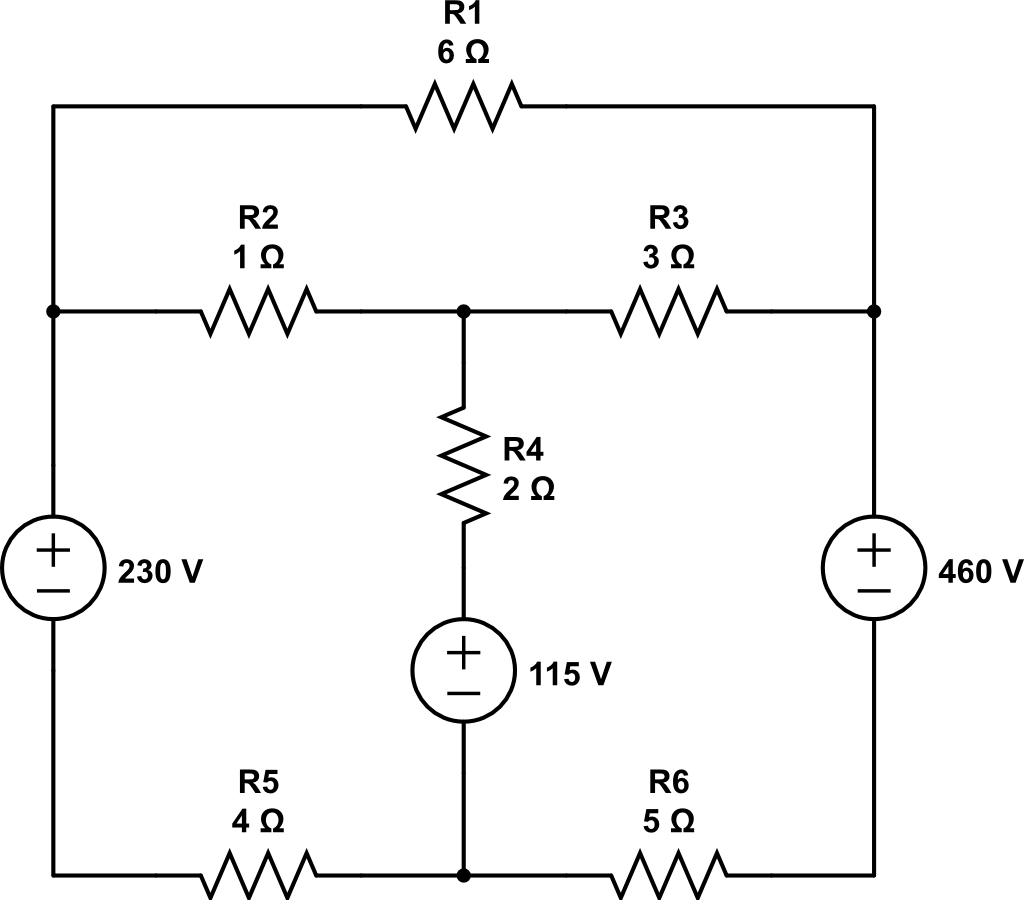
\includegraphics[scale=0.4]{fig4_37.png}
\end{center}
\end{figure}

\begin{enumerate}[(a)]
\item Use the Mesh-Current method to find the total power developed in the circuit.
\item Check your answer by showing that the total power developed equals the total power dissipated.
\end{enumerate}


\vspace{0.1in}

{\bf Question 2} [4] %P4-40

For the following circuit:

\begin{figure}[h!]
\begin{center}
 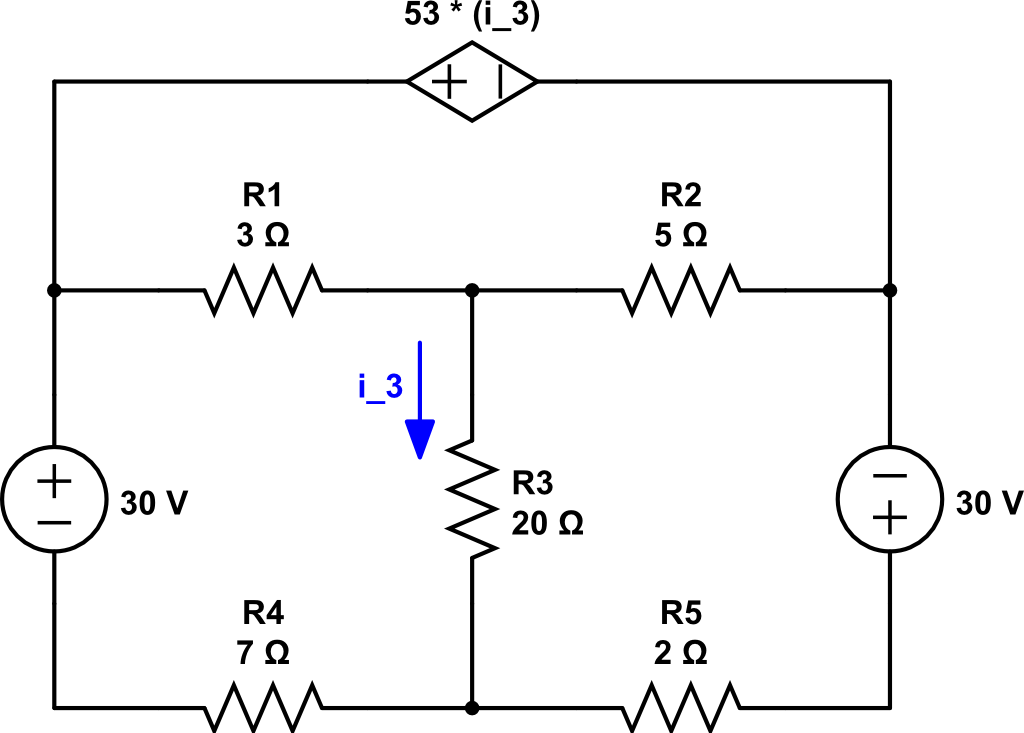
\includegraphics[scale=0.4]{fig4_40.png}
\end{center}
\end{figure}

Use the Mesh-Current method to find the total power developed in the circuit.

\newpage

{\bf Question 3 [4]} % P4-45

For the following circuit:

\begin{figure}[h!]
\begin{center}
 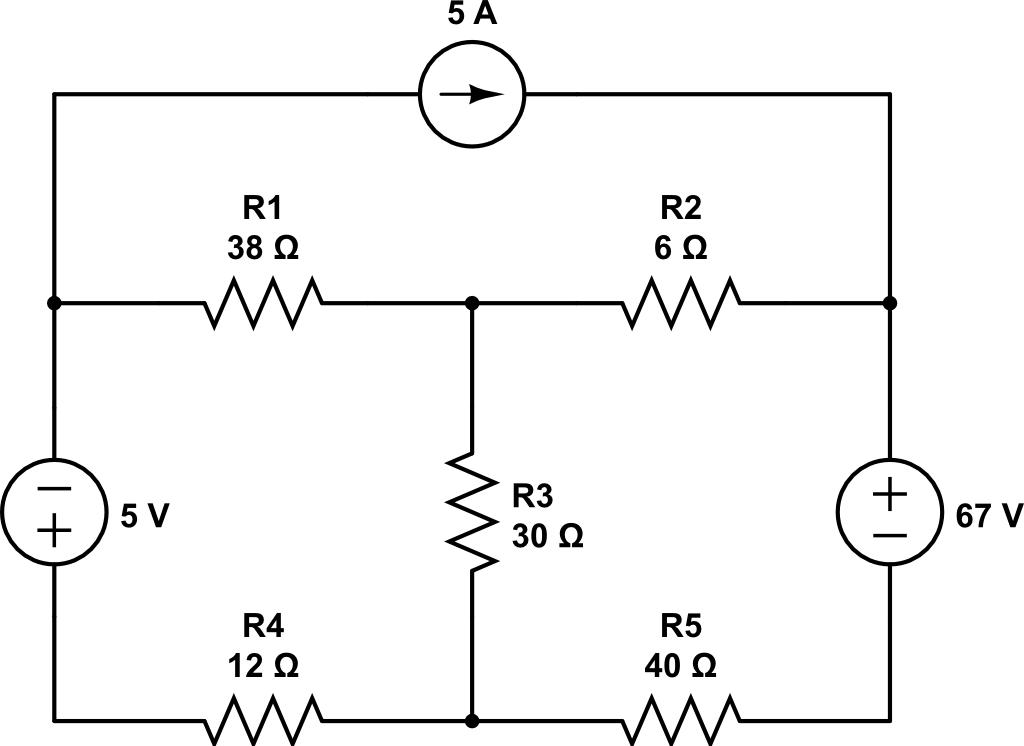
\includegraphics[scale=0.4]{fig4_45.png}
\end{center}
\end{figure}

\begin{enumerate}[(a)]
\item Use the Mesh-Current method to determine the amount of power the 5A current source delivers to the circuit.
\item Find the total power developed in the circuit.
\item Check your answer by showing that the total power developed equals the total power dissipated.
\end{enumerate}

{\bf Question 4} [4] % P4-67

Find the Thevenin Equivalent with respect to Terminals A and B for:

\begin{figure}[h!]
\begin{center}
 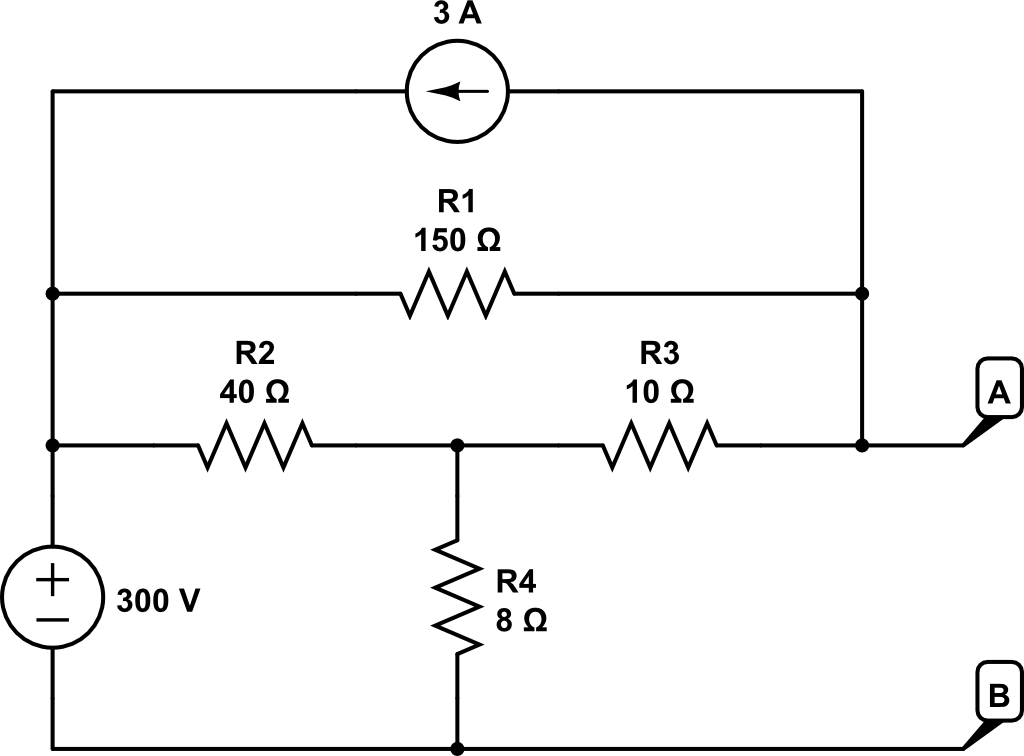
\includegraphics[scale=0.4]{fig4_67.png}
\end{center}
\end{figure}

\newpage

{\bf Question 5} [4] % P4-75

Find the Norton Equivalent with respect to Terminals A and B for:

\begin{figure}[h!]
\begin{center}
 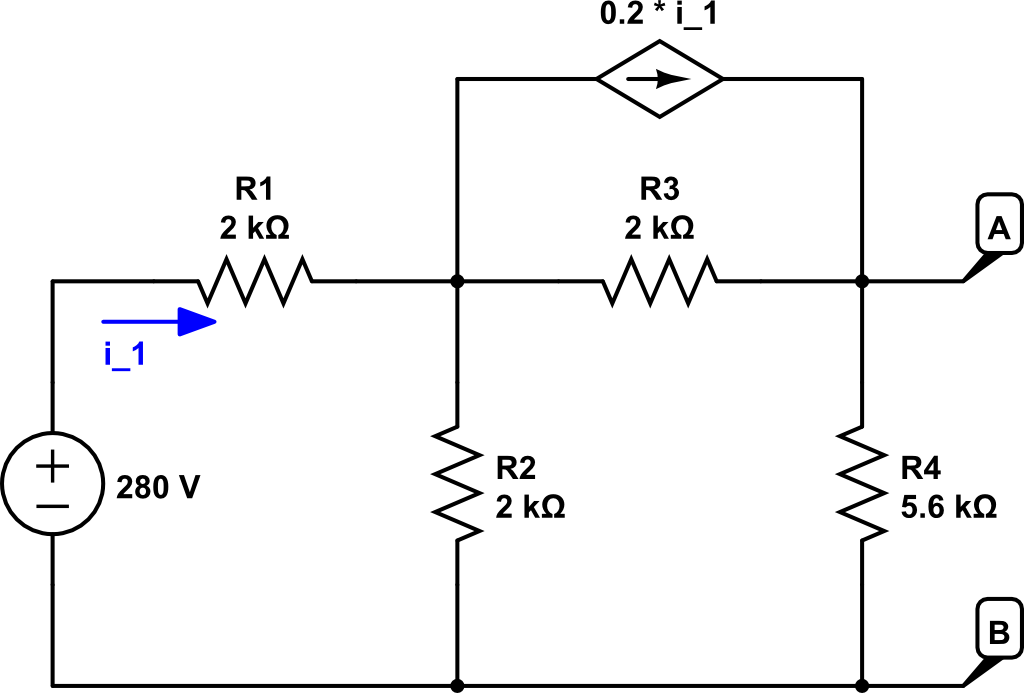
\includegraphics[scale=0.4]{fig4_75.png}
\end{center}
\end{figure}


 
\end{document}
